\section{Hiện thực ứng dụng}
\label{results}

\subsection{Yêu cầu chung của bài toán}
\label{sec4_sub1}
Hệ thống được triển khai là một hệ thống đơn giản, chỉ bao gồm backend và database. Người dùng sử dụng một domain duy nhất truy cập vào ứng dụng. Tùy vị trí của người dùng, ứng dụng được điều hướng đến các server khác nhau. Ứng dụng có sử dụng cân bằng tải. Database có khả năng chịu lỗi cao, thời gian đọc nhanh.

\subsection{Phân tích thiết kế hệ thống}

Với những yêu cầu như đề ra tại \ref{sec4_sub1}, ta nhận định:

\begin{itemize}
    \item Ứng dụng cần một DNS có khả năng phân giải theo khu vực địa lý. Route53 hỗ trợ tính năng này
    \item Ứng dụng có cân bằng tải, Application Load Balancer phù hợp cho trường hợp này. Các loại load balancer khác như network load balancer cũng có thể đảm nhiệm cùng tình năng. Nhưng ở đây ta cần cân bằng tải ở tầng ứng dụng, việc sử dụng tới layer 3 là không cần thiết.
    \item Database trên AWS hầu hết đều cung cấp chức năng replicate. Vì vậy, ta chọn tùy theo tech stack. Ở đây chọn RDS MySQL.
\end{itemize}

Những lựa chọn trên không hẳn là tốt nhất, nhưng được cân nhắc sao cho vừa thể hiện tính phân tán của hệ thống, vừa sử dụng những tài nguyên ít chi phí, đồng thời có khả năng "trình diễn" sâu. Việc sử dụng các dịch vụ server less cũng được cân nhắc, tuy nhiên sẽ trùng đề tài. Khả năng dựng database trên các instance cũng có thể được thực hiện trong trường hợp production để giảm chi phí.

Tổng quan hệ thống trình bày trong hình \ref{fig:sec4-overall-diagram}.

\begin{figure}
    \centering
    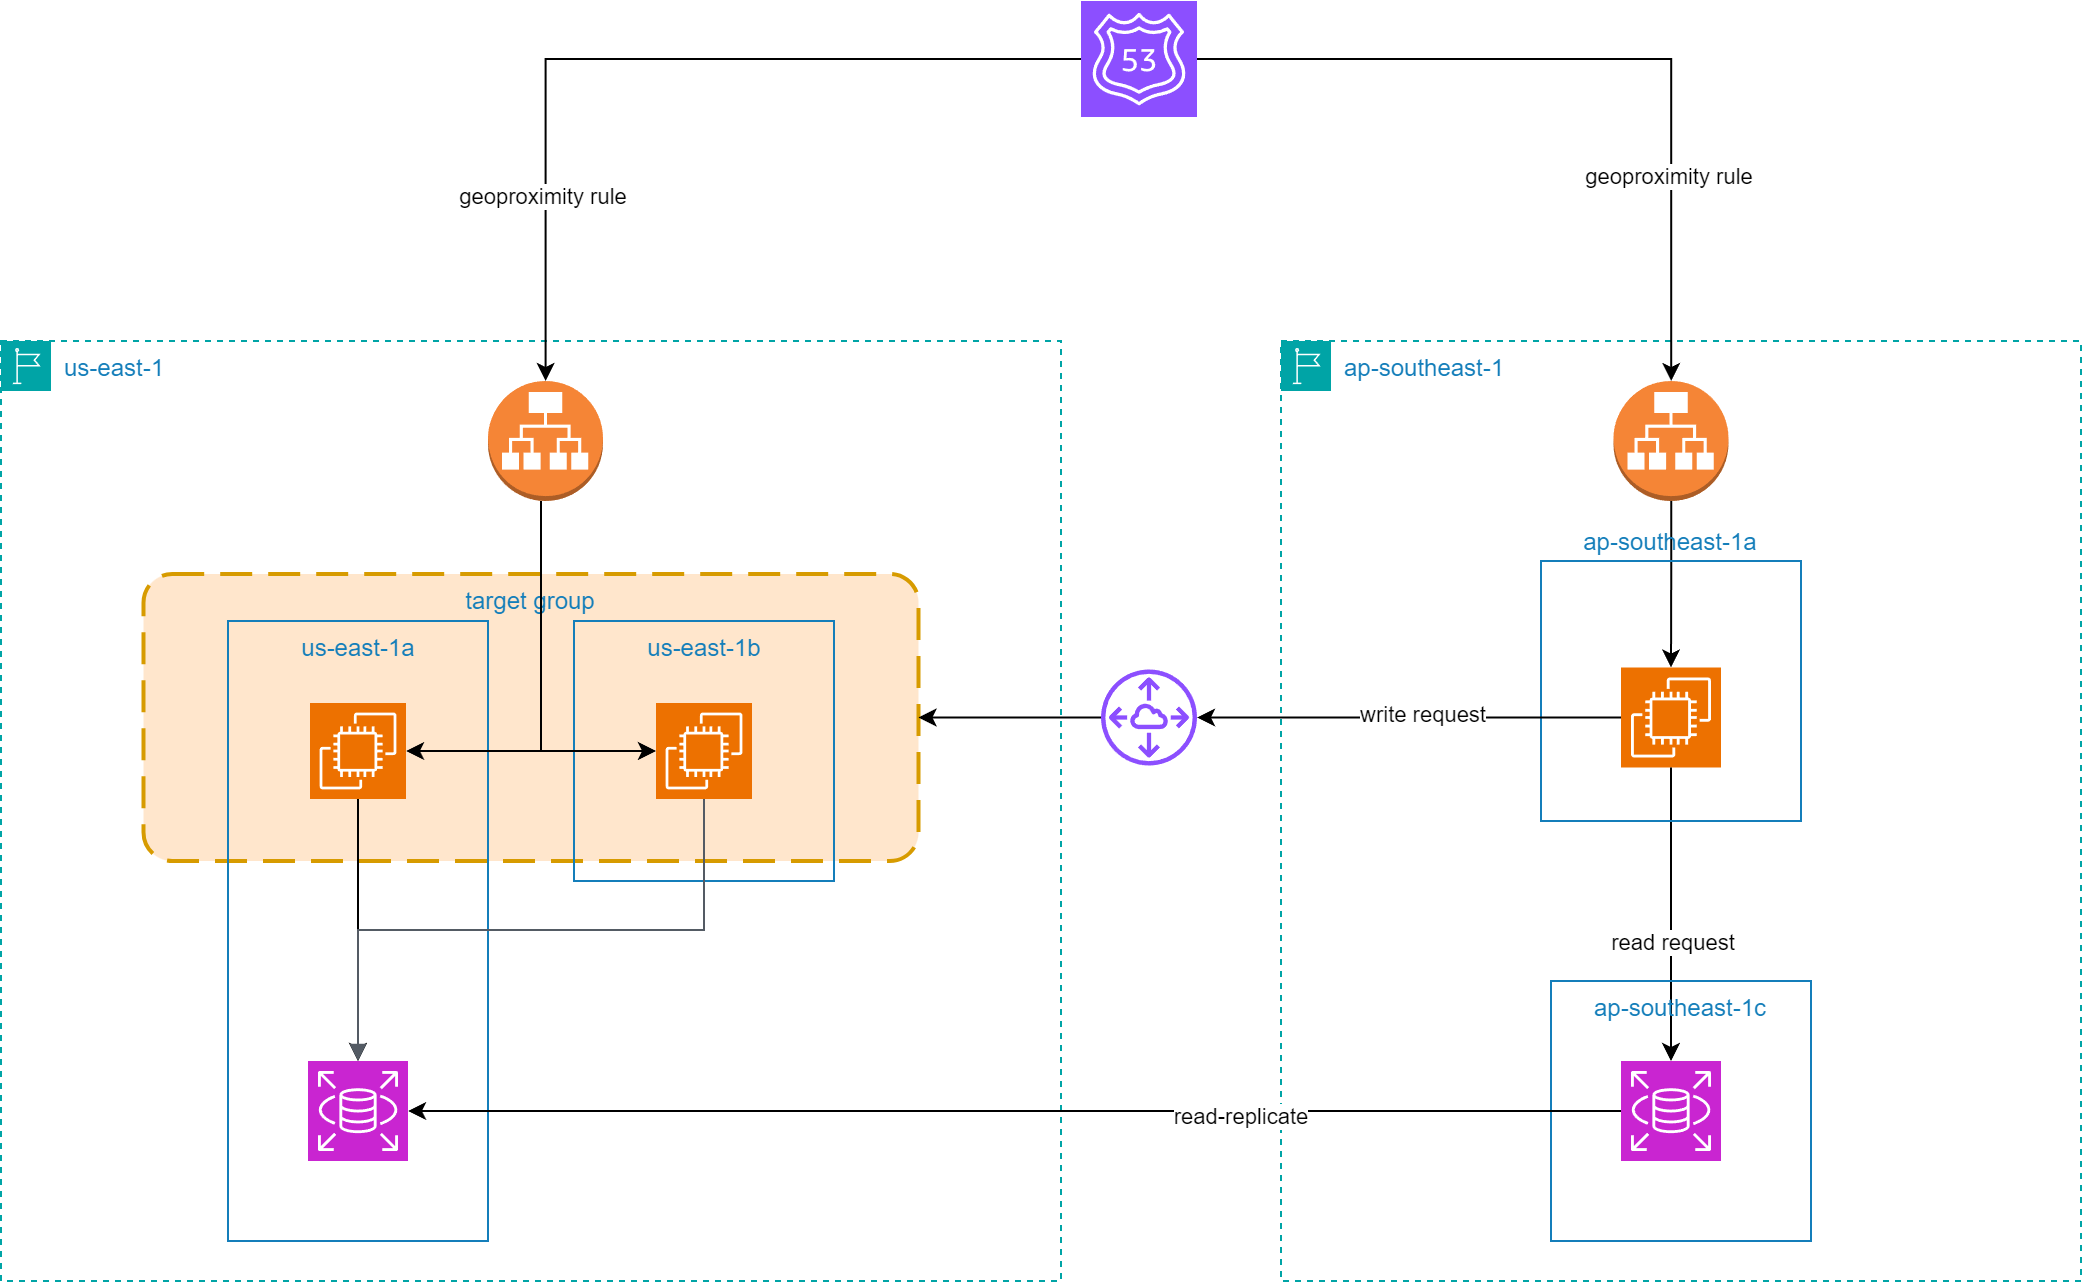
\includegraphics[scale=0.2]{section4/overall-diagram.png}
    \caption{Sơ đồ tổng quan ứng dụng}
    \label{fig:sec4-overall-diagram}
\end{figure}


\begin{figure}
    \centering
    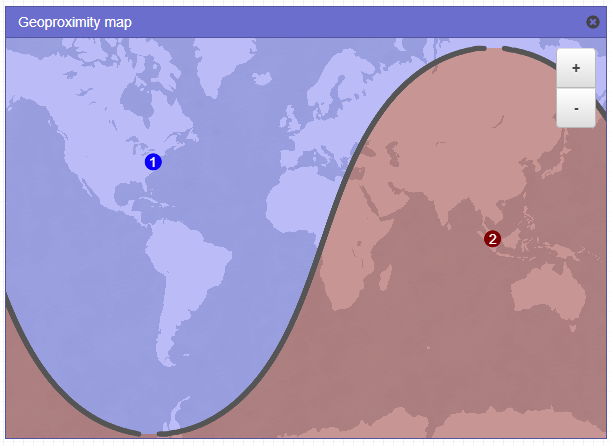
\includegraphics[scale=0.5]{section4/geoproximity_rule.png}
    \caption{Mô tả geoproximity rule của Route 53}
    \label{fig:sec4-geoproximity_rule}
\end{figure}

Tại hình ảnh trên, người dùng sử dụng ứng dụng có domain name được quản lý bởi Route 53. Sử dụng geoproximity policy để điều hướng request tới từng region khác nhau. Nếu địa chỉ IP của người dùng nằm trong vùng màu xanh (số 1), các request sẽ được điều hướng tới region \textit{us-east-1}, ngược lại các request sẽ được xử lý tại region \textit{ap-southeast-1} (xem hình \ref{fig:sec4-geoproximity_rule}).

Tại backend, deploy web service nginx và một service Flask app đơn giản. Ứng dụng này trả về các truy xuất vào các database khi được yêu cầu hoặc trả về hostname của server và timestamp ở mặc định. Trước khi request đi vào backend, sử dụng một Application Load Balancer nhằm cân bằng tải. Nó thực hiện heal check tới backend thông qua port 80 và serve port 80 ra ngoài. Từ bên ngoài không gọi thẳng được tới backend thông qua giao thức http.

Tại database, tiến hành deploy một RDS MySQL chính tại \textit{us-east-1} và một RDS Read Replicate tại \textit{ap-southeast-1} (do chi phí ở \textit{us-east-1} rẻ hơn). AWS hỗ trợ chúng ta đồng bộ dữ liệu cho 2 database này với cam kết cao. Các request yêu cầu database tại \textit{us-east-1} sẽ được xử lý trên RDS Master. Trong khi các request đọc database ở \textit{ap-southeast-1} sẽ được đọc trên RDS Slave. Các yêu cầu ghi database tại \textit{ap-southeast-1} được chuyển tiếp tới backend ở \textit{us-east-1} thông qua một private connection (VPC Peering connection)

\subsection{Hiện thực ứng dụng}



\subsection{Kết quả ứng dụng trong từng ngữ cảnh}